\hypertarget{system-design}{%
\chapter{System Design}\label{system-design}}

\begin{draftnote}

\textbf{Draft status, 04 November 2026.} The five figures referenced
here are committed in \texttt{docs/diagrams/} as Mermaid sources with
rendered \texttt{.svg} (vector, for LaTeX) and \texttt{.png} at 2\texttimes{} (for
slides). Each has a regenerable source beside it, so no figure in this
report is one nobody can reproduce --- the same rule the measurements
folder works under. \textbf{These are the figures the viva will be
conducted from}, so they are worth knowing better than this chapter's
prose.

\end{draftnote}

\begin{center}\rule{0.5\linewidth}{0.5pt}\end{center}

\hypertarget{architecture}{%
\section{Architecture}\label{architecture}}

\begin{figure}[htbp]
\centering
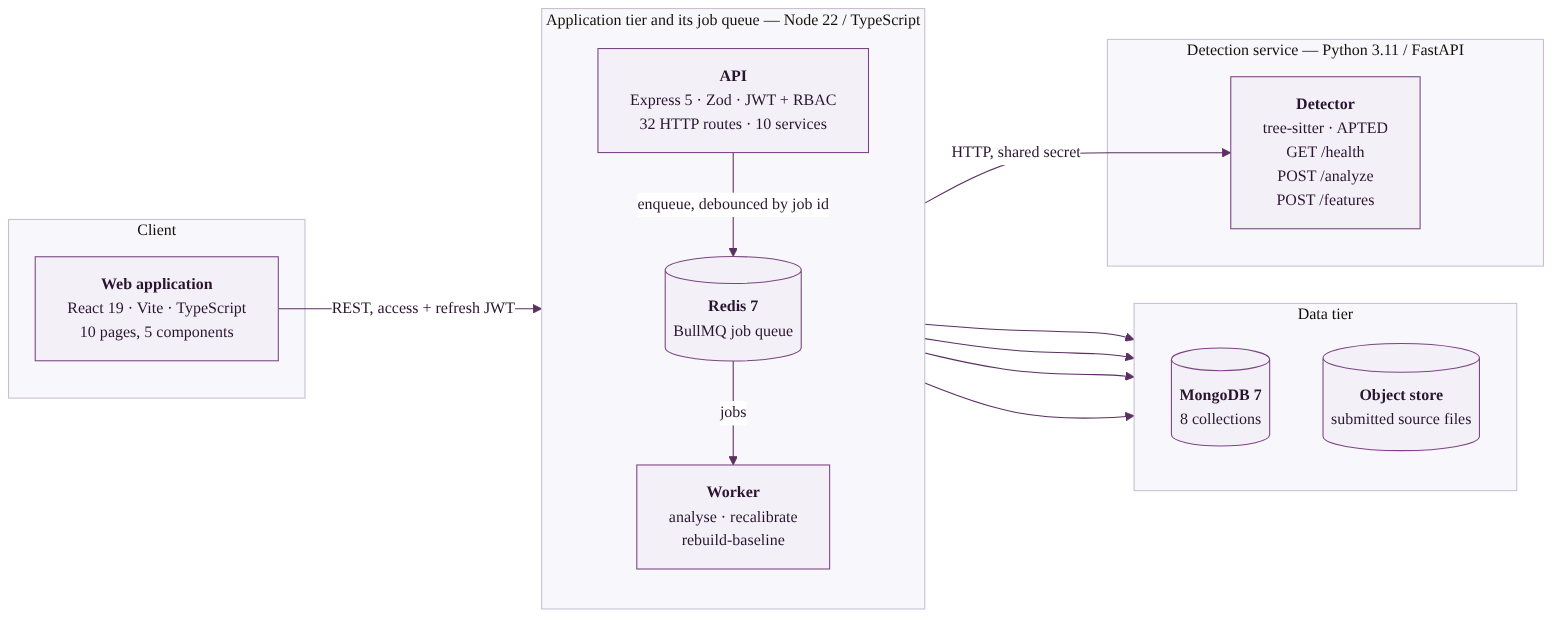
\includegraphics[width=\linewidth,height=0.78\textheight,keepaspectratio]{figures/01-architecture.png}
\caption{System architecture: three tiers and one detection service. The web application never talks to the detector or to any data store; everything goes through the API, which holds the only credentials.}
\label{fig:01-architecture}
\end{figure}

Three tiers and one detection service.

\textbf{The web application never talks to the detector or to any data
store.} Everything goes through the API, which holds the only
credentials in the system. That is the single most important property of
the diagram and the one to point at first: there is exactly one tier
where a credential exists, exactly one tier that can reach MongoDB,
Redis or the object store, and exactly one place where an authorisation
decision is made.

Redis is drawn inside the application tier to keep the queue flow
legible, but it is infrastructure and runs as its own container
alongside MongoDB and the object store.

\textbf{The worker is the same codebase as the API, started on a
different entry point.} A queued job and a synchronous request therefore
share one set of services rather than two implementations that can drift
apart. Two copies of the scoring logic would eventually disagree, and
the disagreement would surface as a result nobody could reproduce.

The split between the API and the detector deserves defending, because
it looks like unnecessary complexity for a student project. It is not.
The parsing ecosystem this system depends on --- tree-sitter grammars
and an APTED implementation --- is Python. The web application and its
document model are far more naturally written in TypeScript against
Mongoose. Rather than compromise one to accommodate the other, the
detector is a \textbf{stateless} HTTP service that parses and compares,
and every piece of state stays in the API.

\hypertarget{one-submission-end-to-end}{%
\section{One submission, end to end}\label{one-submission-end-to-end}}

\begin{figure}[htbp]
\centering
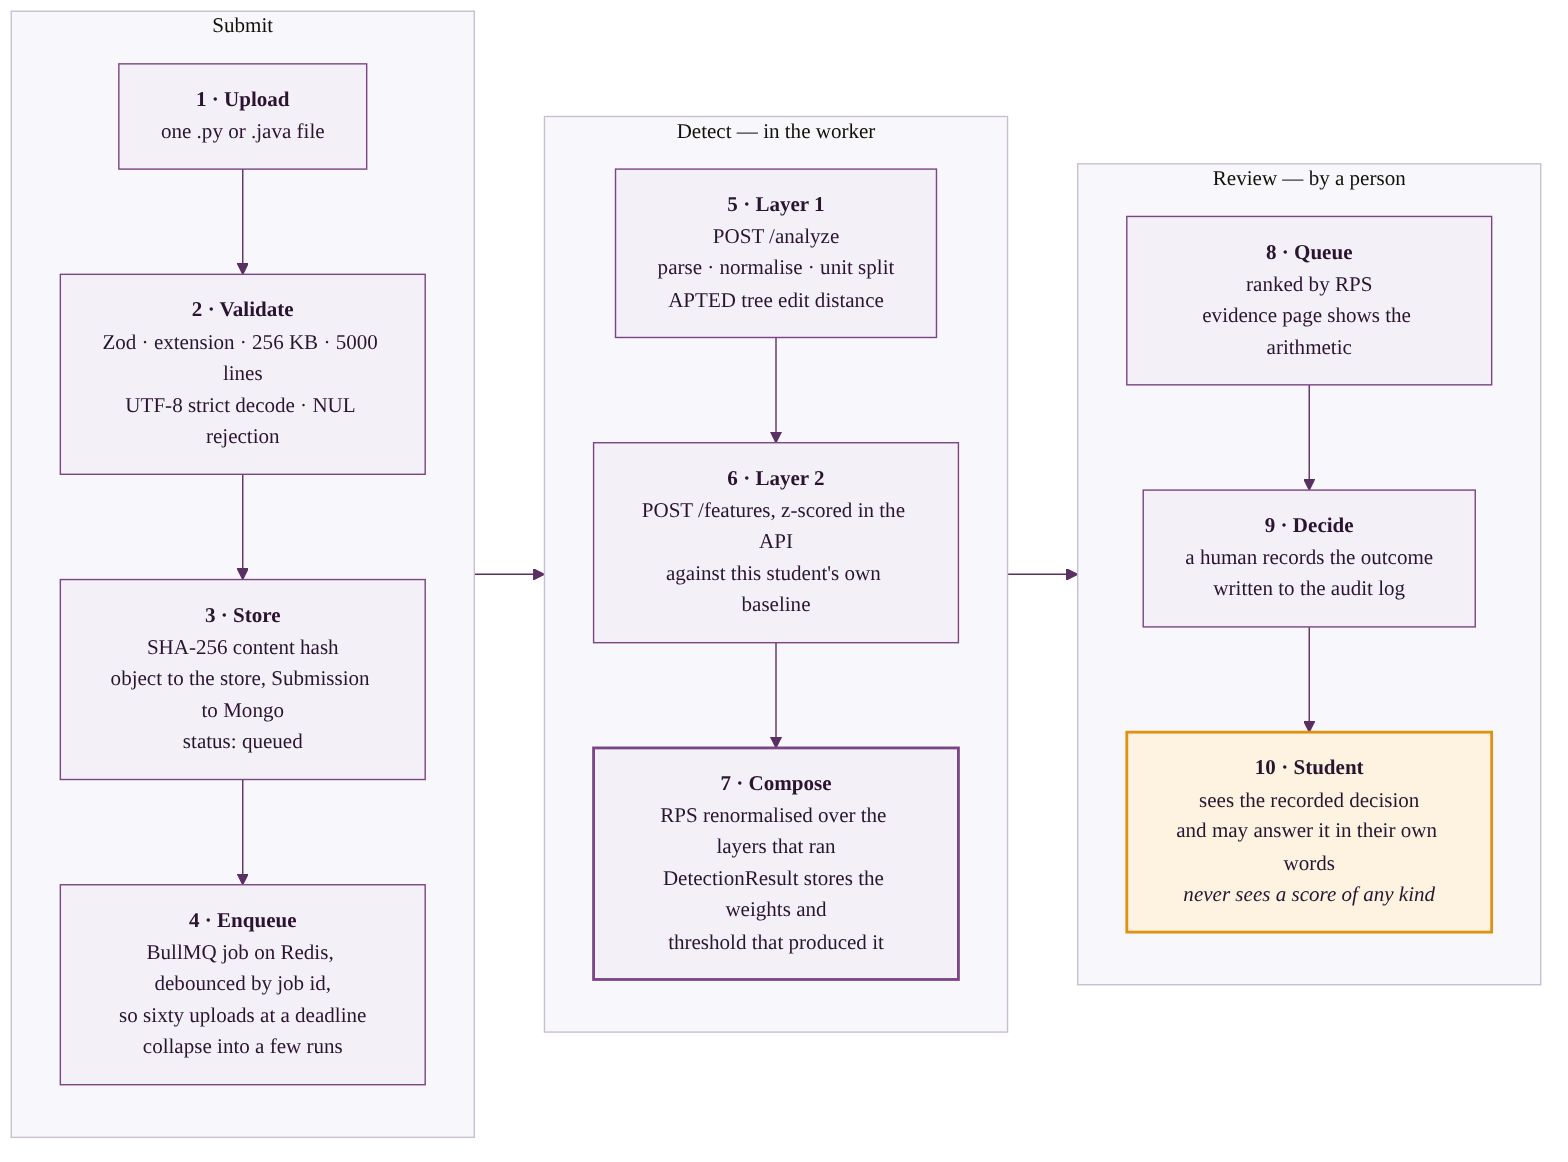
\includegraphics[width=\linewidth,height=0.78\textheight,keepaspectratio]{figures/02-data-flow.png}
\caption{One submission, end to end. Step 4 is debounced by job identity; step 7 stores the weights and threshold that produced the score; step 10 shows the student a decision and never a score.}
\label{fig:02-data-flow}
\end{figure}

Ten steps across three phases: upload, detection, review.

Three of the steps carry design decisions rather than mechanism.

\textbf{Step 4 is debounced by job identity.} Sixty uploads arriving at
a deadline collapse into a handful of detection runs rather than sixty,
because each run reads the current cohort anyway. Detection is slow ---
it parses, compares against candidates and waits on a second service ---
so performing it inside the upload request would make uploads take
seconds and fail under load at precisely the moment every student
submits at once.

\textbf{Step 7 stores the weights and the review threshold that produced
the score, on the result itself.} This is what lets the evidence page
stay readable after the configuration changes. Without it, a result
opened next term would be rendered against whatever weights happen to be
current, and its arithmetic would no longer add up.

\textbf{Step 10 is a design decision, not an omission.} The student sees
the recorded decision and may answer it, and never sees a score, because
a ranking a student can read is a ranking a student can tune against.

\hypertarget{data-model}{%
\section{Data model}\label{data-model}}

\begin{figure}[htbp]
\centering
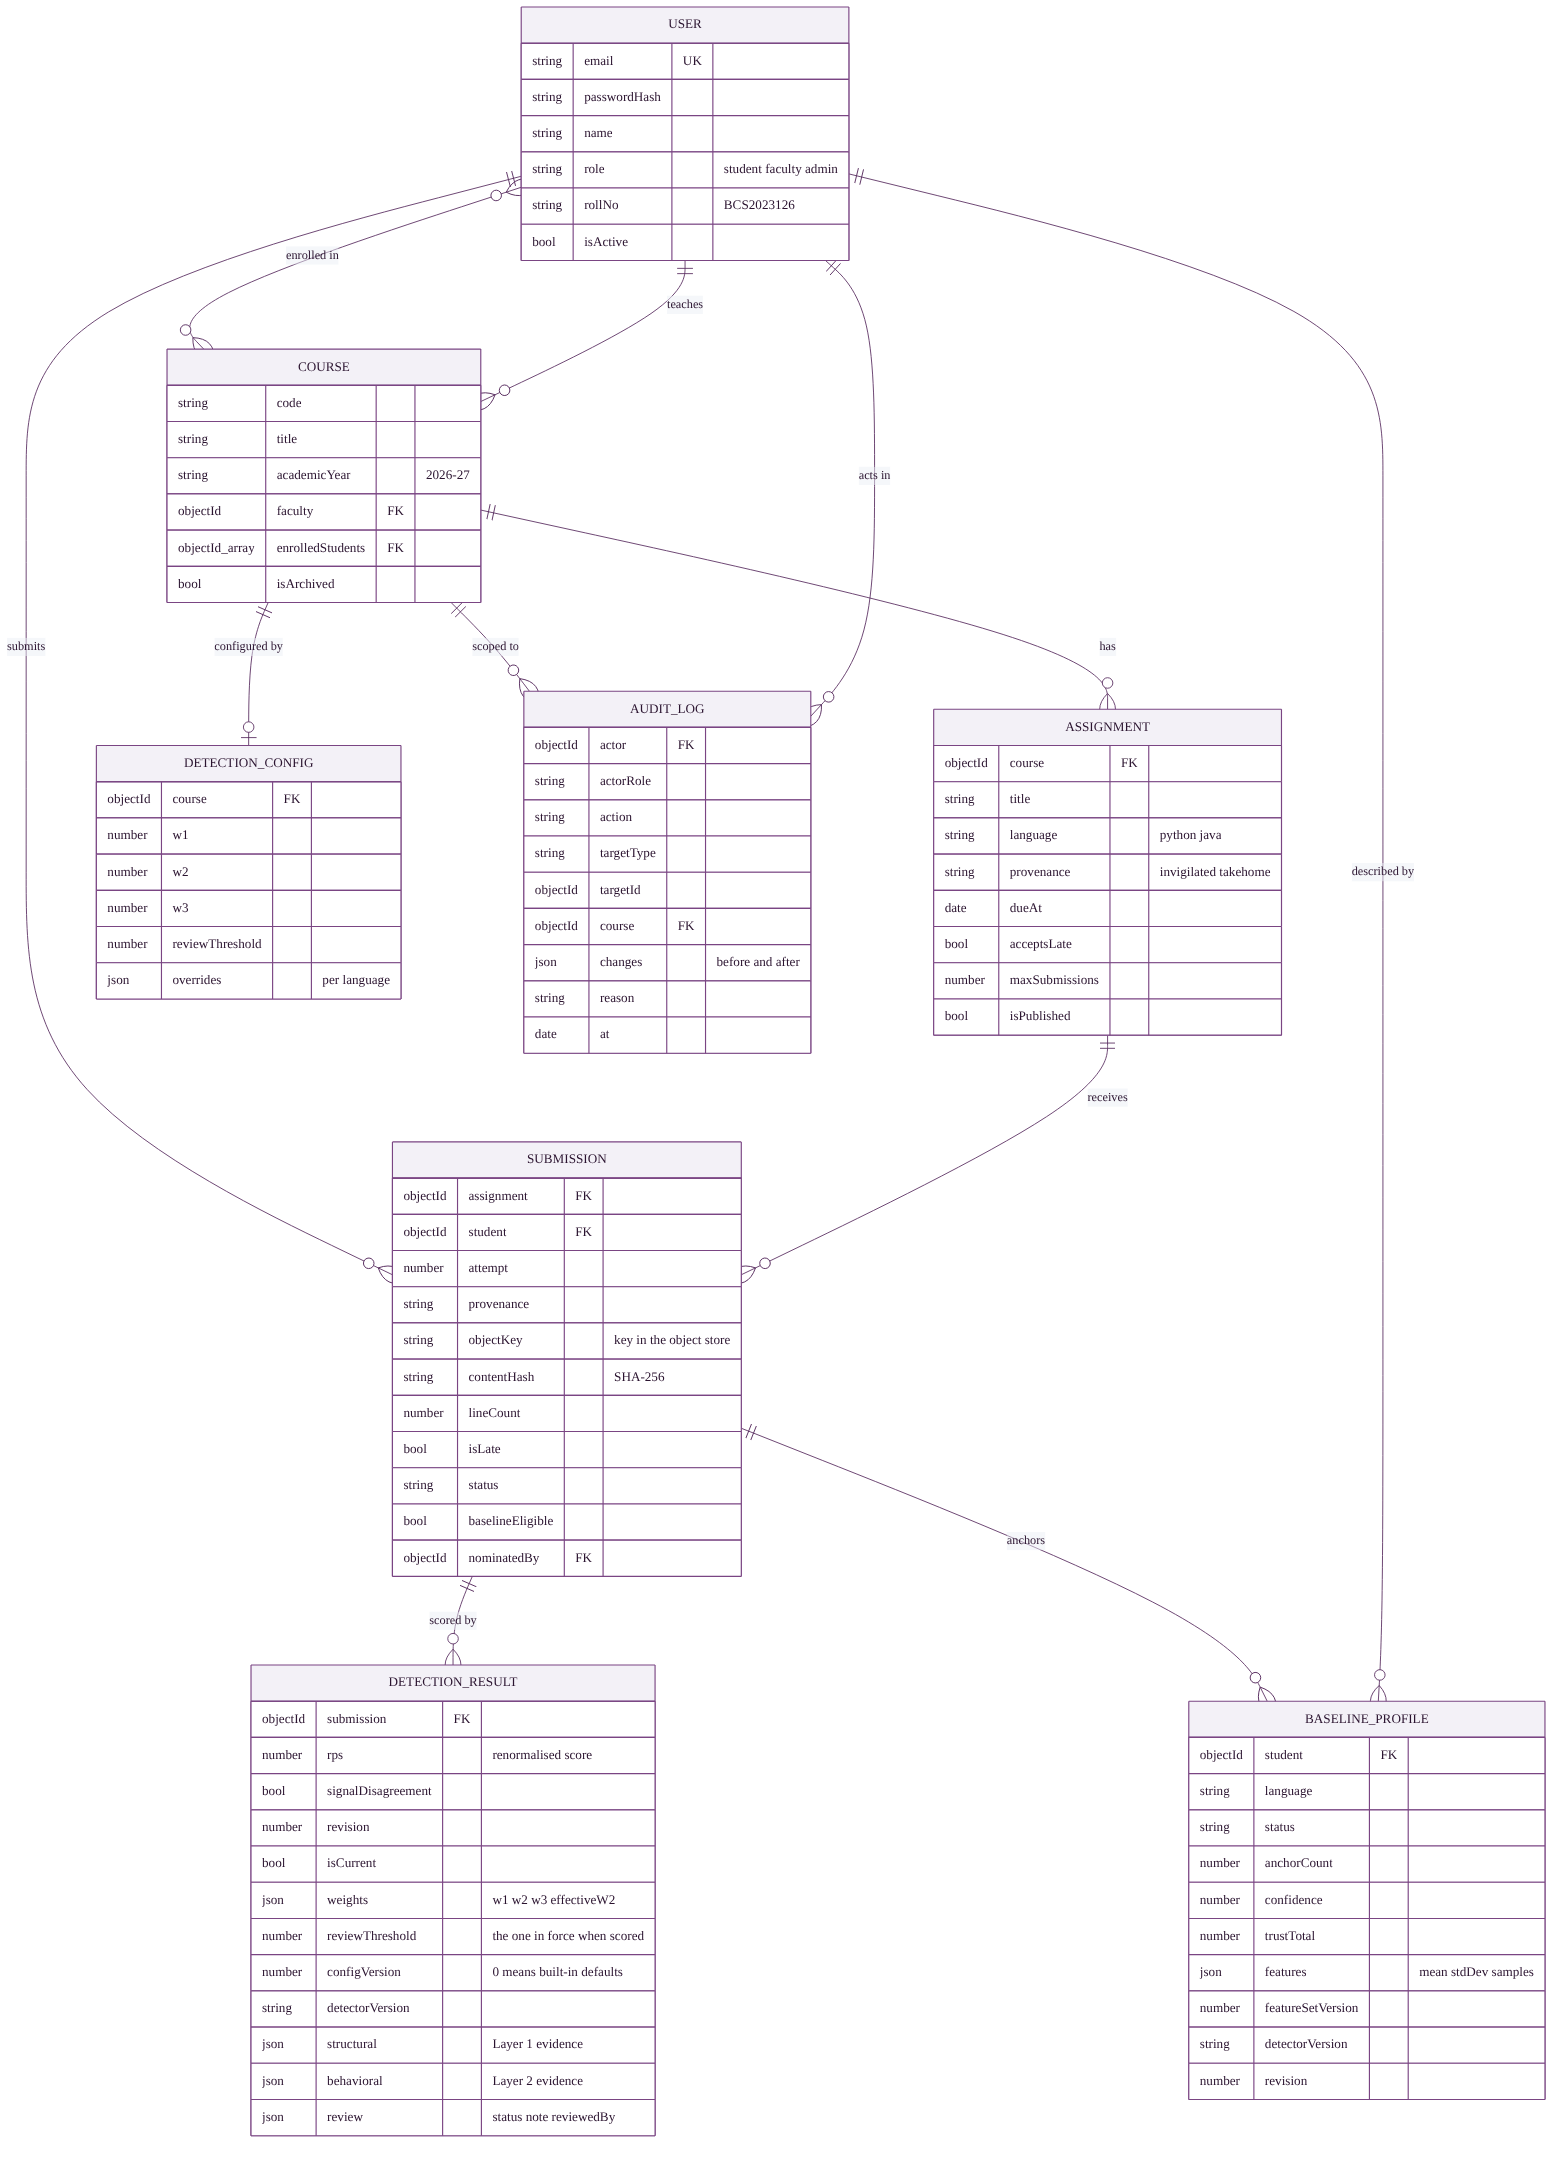
\includegraphics[width=\linewidth,height=0.78\textheight,keepaspectratio]{figures/03-data-model.png}
\caption{The eight collections. DetectionResult carries both layers' evidence rather than only their scores, and AuditLog is separate from the documents it describes.}
\label{fig:03-data-model}
\end{figure}

Eight collections: \texttt{User}, \texttt{Course}, \texttt{Assignment},
\texttt{Submission}, \texttt{DetectionResult}, \texttt{DetectionConfig},
\texttt{BaselineProfile} and \texttt{AuditLog}.

Three properties of the model are the ones to explain.

\textbf{\texttt{DetectionResult} carries both layers' evidence, not
merely their scores.} That is what makes the evidence page reproducible
from stored data rather than recomputed on demand. A score alone is an
assertion; the evidence beside it is what a reviewer can actually act on
and a student can contest.

\textbf{\texttt{isCurrent} and \texttt{revision} mean a re-run
supersedes a result without destroying it.} A decision may already have
been recorded against the earlier result, and destroying it would orphan
that decision.

\textbf{\texttt{AuditLog} is separate from the documents it describes},
so that the record of who changed what cannot be edited by the same
operation that changes the thing. An audit log a privileged operation
can rewrite is not an audit log.

\hypertarget{the-layer-2-pipeline}{%
\section{The Layer 2 pipeline}\label{the-layer-2-pipeline}}

\begin{figure}[htbp]
\centering
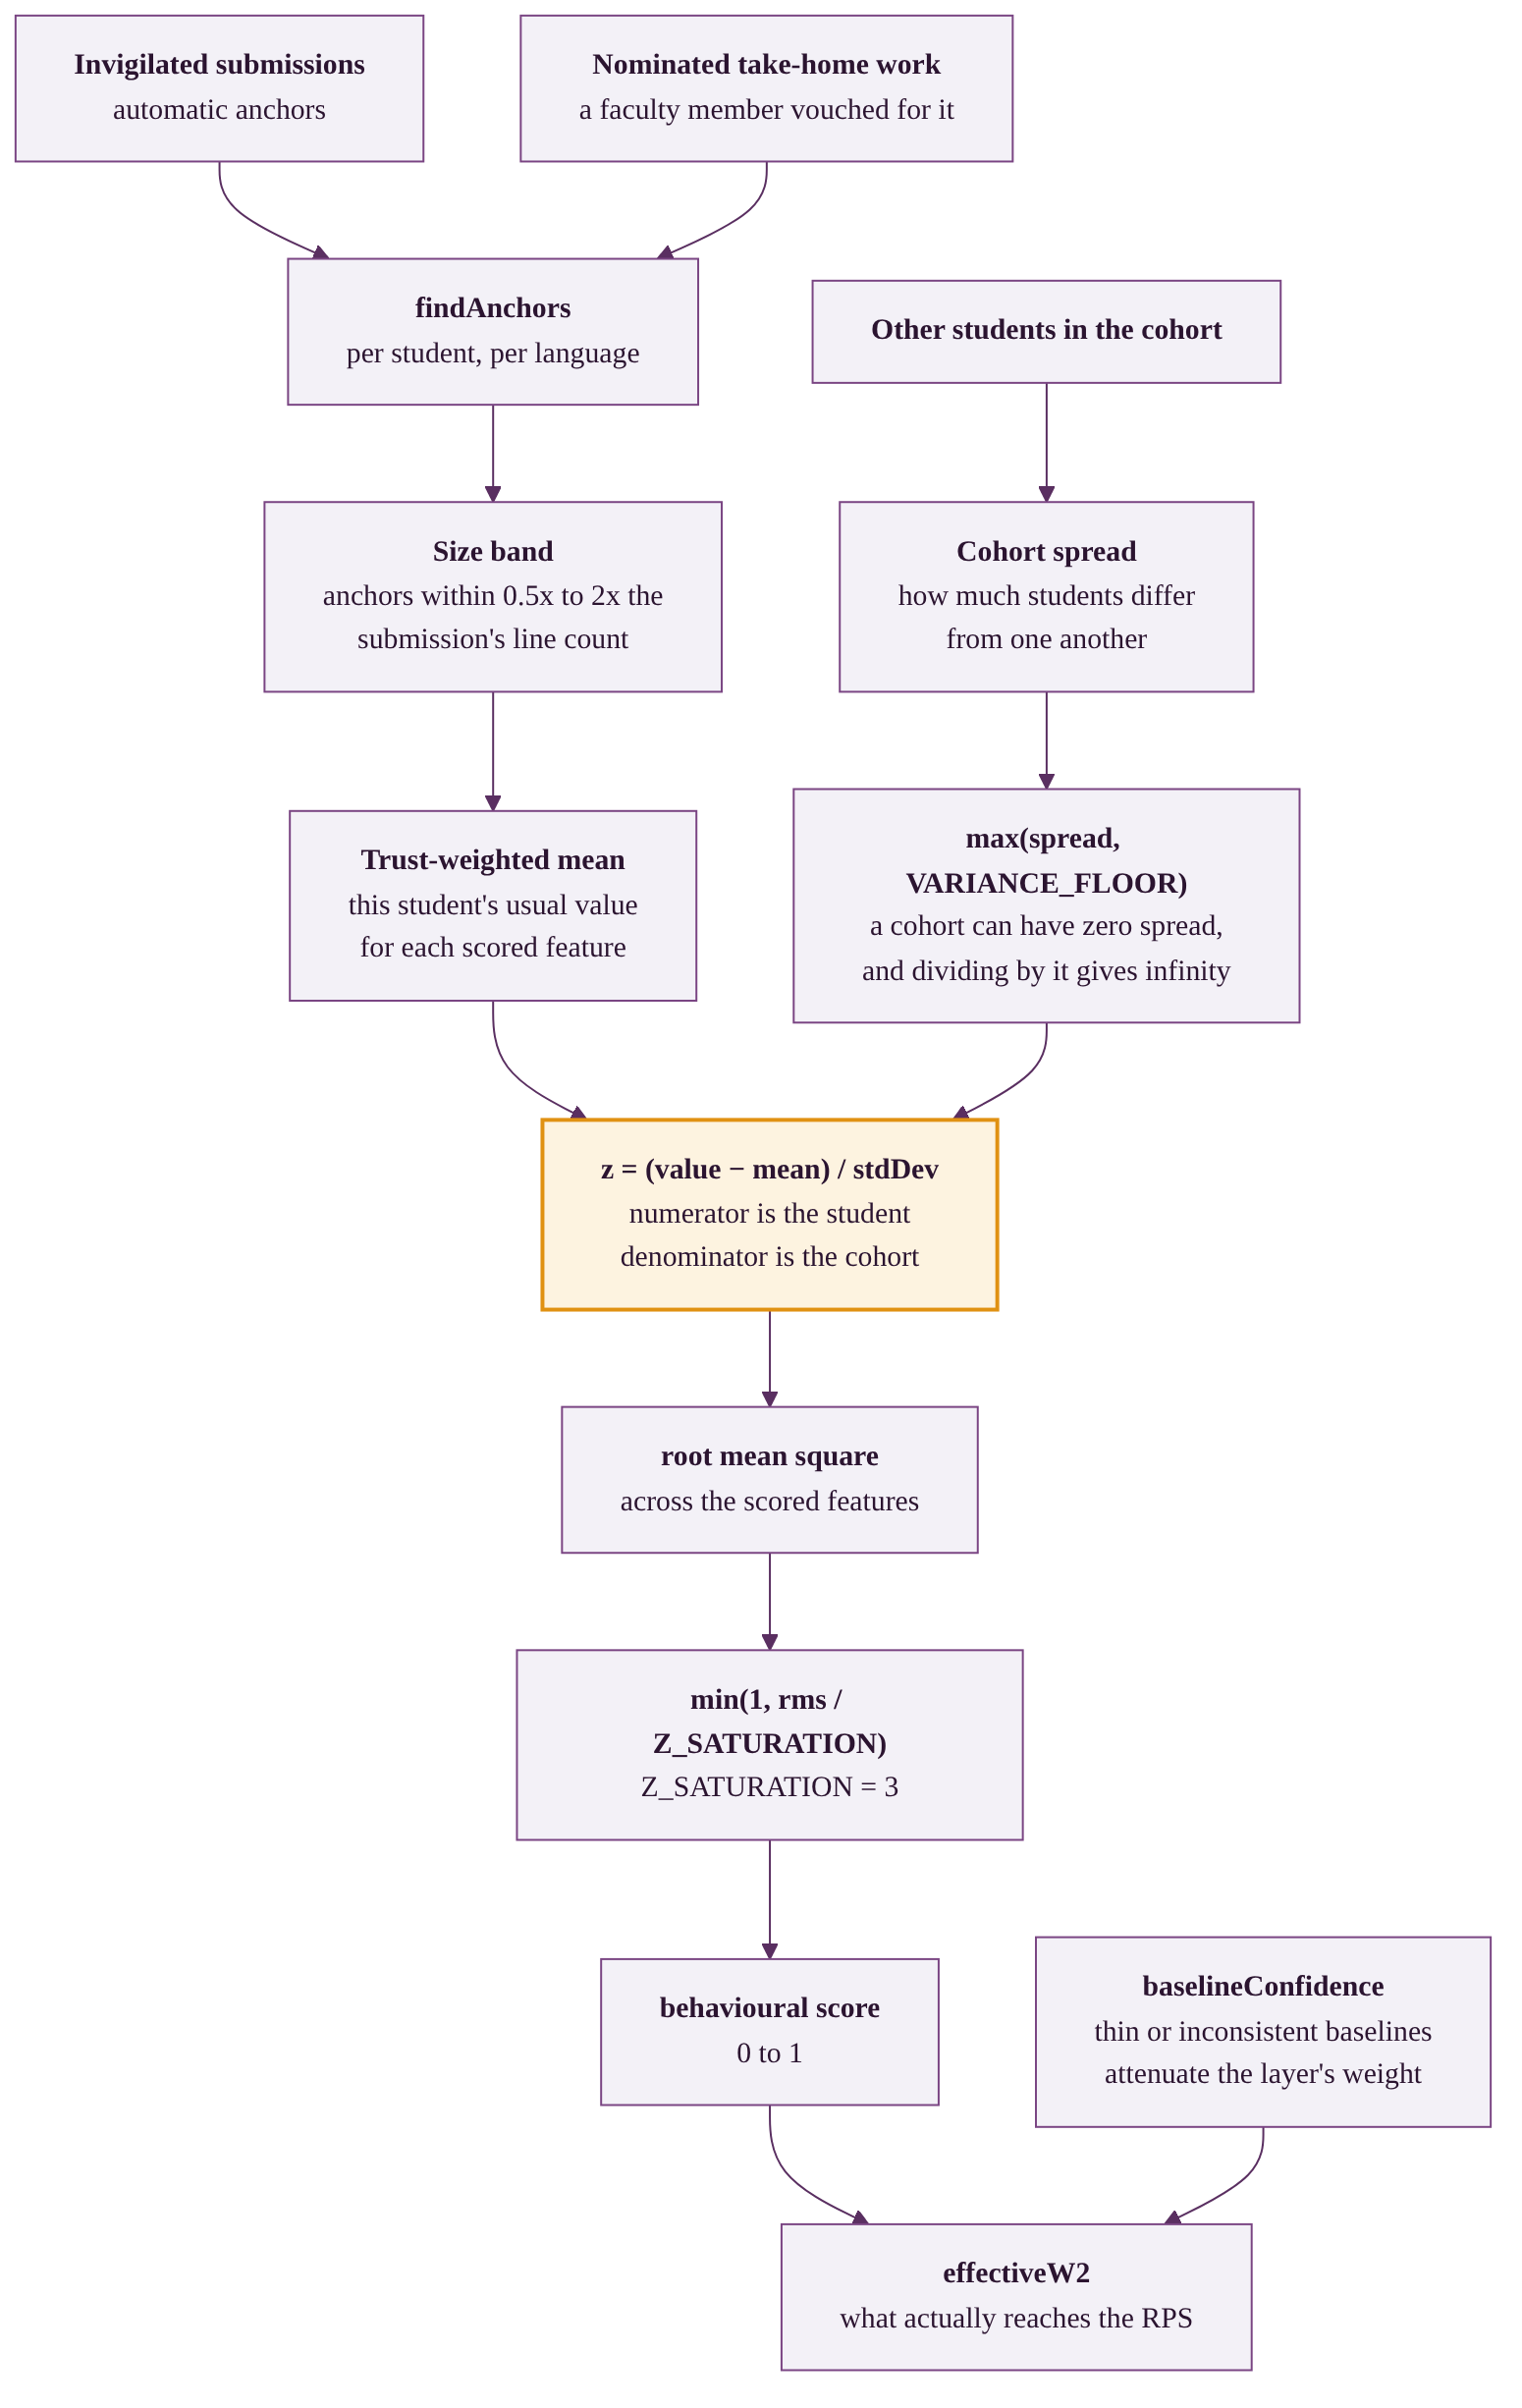
\includegraphics[width=\linewidth,height=0.78\textheight,keepaspectratio]{figures/04-layer2-pipeline.png}
\caption{The Layer 2 pipeline. The numerator comes from the student's own anchors, trust-weighted; the denominator comes from the cohort, floored.}
\label{fig:04-layer2-pipeline}
\end{figure}

This is the project's research contribution in one figure, and the first
place to look when defending it.

Note what joins at the z-score, because it is the thing most often
misread --- including in this project's own earlier documentation:

\begin{itemize}
\tightlist
\item
  the \textbf{numerator} comes from the student's own anchors,
  trust-weighted;
\item
  the \textbf{denominator} comes from the \textbf{cohort}, floored.
\end{itemize}

A z here means \emph{how far this submission sits from this student's
usual, measured in units of how much students in this class differ from
one another.} Both halves are load-bearing, and an earlier version of
the project documentation claimed the comparison was ``never against the
cohort'', which is false and would not survive an examiner opening the
file.

The floor exists because a cohort can produce zero spread on a coarse
feature, and dividing by zero gives infinity.

\textbf{The justification for the cohort denominator is an argument, not
a measurement, and the report must present it as such.} The argument is
that a student's own spread, estimated from three or four anchors, is
too unstable to divide by: a mean is personal, whereas a spread is
closer to a property of the feature. An AUC comparison previously quoted
in support of this has been retracted --- it is traceable to no run in
the measurements folder (Chapter 7 \S{}7.4) --- so the design choice stands
on its reasoning alone.

\hypertarget{composing-the-review-priority-score}{%
\section{Composing the Review Priority
Score}\label{composing-the-review-priority-score}}

\begin{figure}[htbp]
\centering
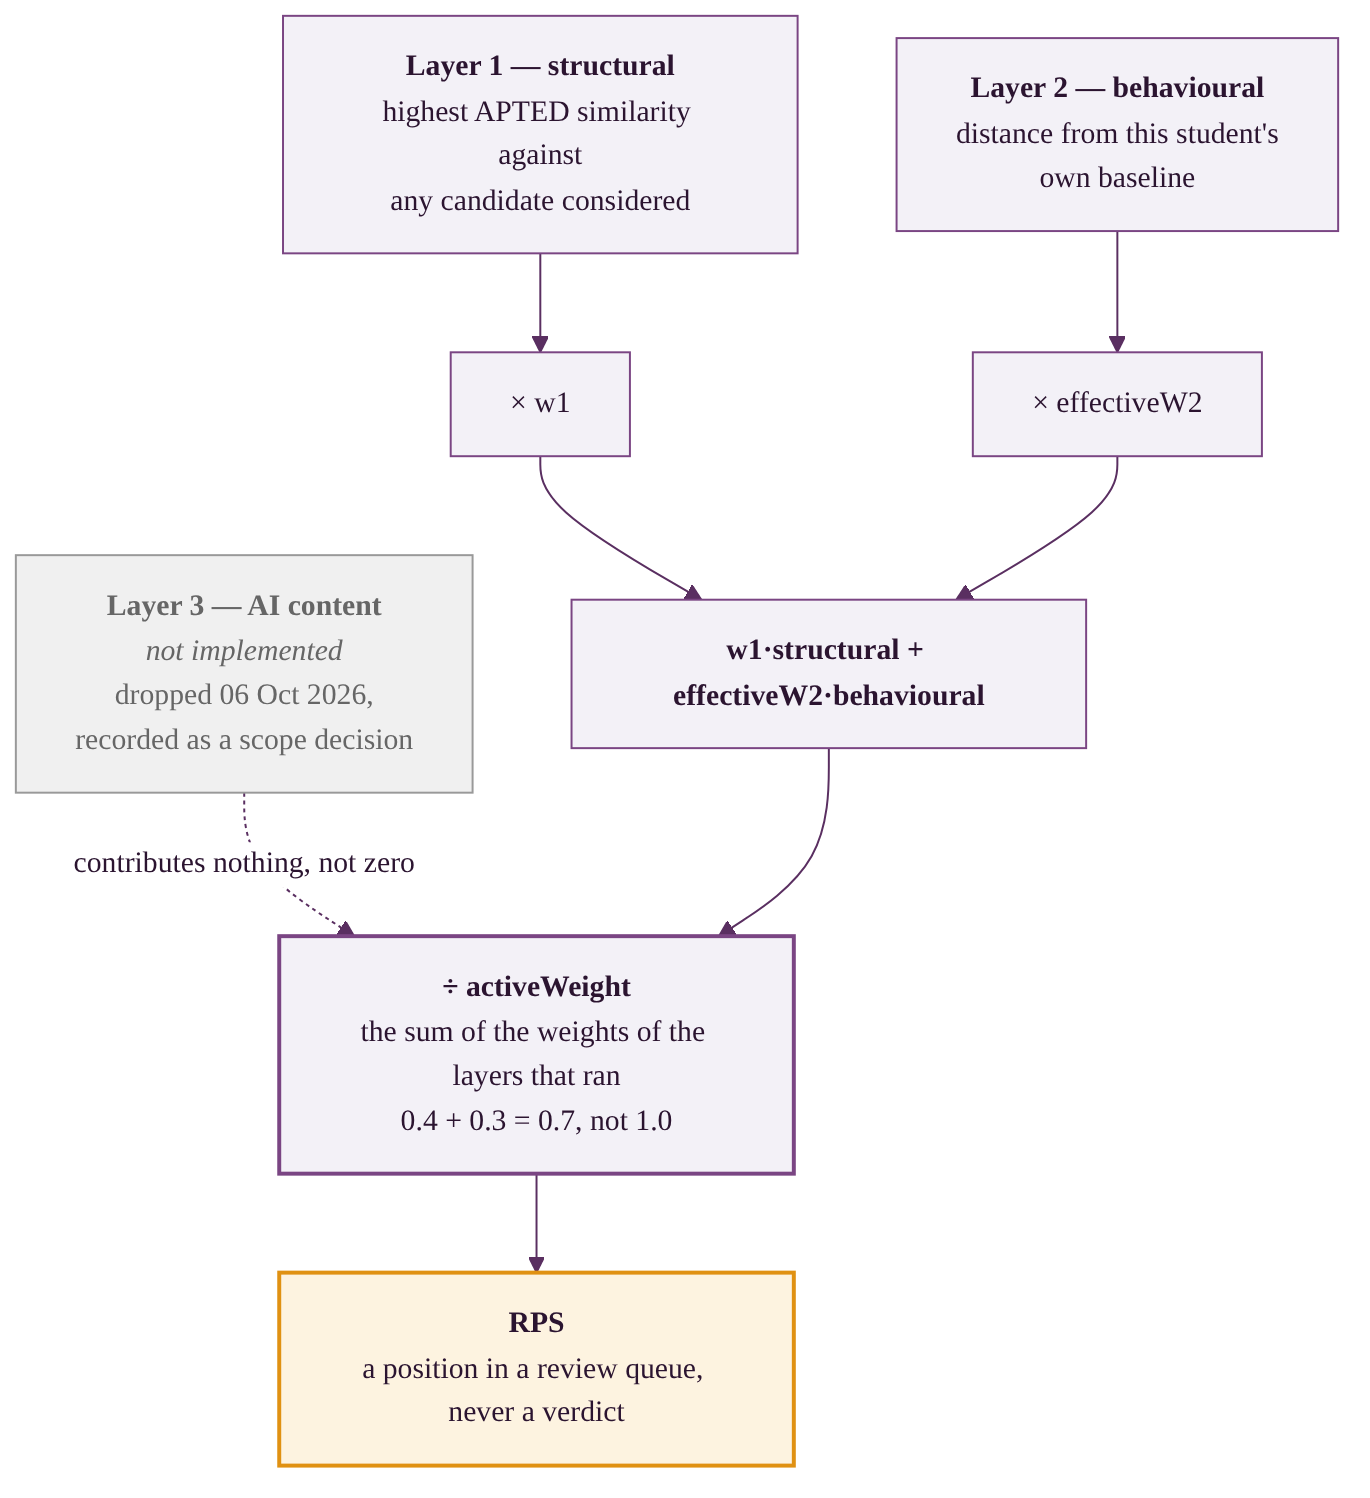
\includegraphics[width=\linewidth,height=0.78\textheight,keepaspectratio]{figures/05-rps-composition.png}
\caption{Composing the RPS. With Layer 3 absent the divisor is 0.7, so the configured 0.4/0.3/0.3 act as 0.571/0.429. An absent layer contributes nothing, not zero.}
\label{fig:05-rps-composition}
\end{figure}

\begin{verbatim}
activeWeight = (structuralOk ? w1 : 0) + (behaviouralOk ? effectiveW2 : 0)
RPS          = (w1 \textperiodcentered{} structural + effectiveW2 \textperiodcentered{} behavioural) / activeWeight
\end{verbatim}

\textbf{With Layer 3 absent, the configured weights 0.4 / 0.3 / 0.3 are
never the applied ones.} The divisor is the sum of the weights of the
layers that actually ran, which is 0.7, so they act as \textbf{0.571 /
0.429}. Quoting the configured triple as the operative weights would be
wrong, and the evidence page renders the renormalisation explicitly for
exactly this reason.

\textbf{An absent layer contributes nothing rather than contributing
zero}, because zero is a finding and an absent layer has made no
finding. Treating absence as zero would drag every score down by a third
and make a two-layer result incomparable with a three-layer one.

\texttt{effectiveW2} is Layer 2's weight after attenuation by baseline
confidence, so a thin baseline reduces the layer's influence instead of
being trusted at full strength. Figure 5 shows Layer 3 greyed and
excluded rather than omitted, because its absence is what makes the
renormalisation necessary.

\hypertarget{baseline-integrity-as-a-design-concern}{%
\section{Baseline integrity as a design
concern}\label{baseline-integrity-as-a-design-concern}}

Layer 2's failure mode is not a missed detection. It is a \textbf{wrong
baseline accusing an honest student}, and the design carries five
mitigations for it:

\begin{enumerate}
\def\labelenumi{\arabic{enumi}.}
\tightlist
\item
  \textbf{Anchor provenance} --- only invigilated work, or work a
  student nominates and faculty accept, may describe their style.
\item
  \textbf{Minimum anchor count} --- below three, the layer declines to
  score rather than guessing.
\item
  \textbf{Baseline confidence} --- a thin or inconsistent baseline
  attenuates the layer's weight instead of being trusted at full
  strength.
\item
  \textbf{Low-variance flag} --- a student whose own work varies less
  than the cohort's is penalised by z-scoring, and the result says so.
\item
  \textbf{Cohort saturation flag} --- when the pooled spread collapses,
  every z-score is a real difference divided by an invented floor, and
  the layer has stopped discriminating. The result says that too.
\end{enumerate}

Mitigations 2 to 5 share a character worth naming in the report:
\textbf{the system reports that it cannot tell, rather than producing a
number that looks like an answer.} That is what an evidence system owes
a reviewer, and it is the design-level expression of the principle in
Chapter 2 \S{}2.2 that a tool does not determine plagiarism.

\hypertarget{what-the-diagrams-deliberately-do-not-show}{%
\section{What the diagrams deliberately do not
show}\label{what-the-diagrams-deliberately-do-not-show}}

These figures show the system that exists, not the system the project
presentation describes. Three items in that deck are absent here because
they are absent in the code, and the report carries them as scope
decisions rather than letting an examiner find the gap:

\begin{itemize}
\tightlist
\item
  \textbf{Layer 3, CodeBERT.} Dropped 06 October 2026. Figure 5 shows it
  greyed and excluded rather than omitting it, because its absence is
  what makes the renormalisation necessary. The reasoning is in Chapter
  5 \S{}5.4.
\item
  \textbf{The WebSocket push.} Not built. The queue is polled by the
  reviewer rather than pushed to them.
\item
  \textbf{The side-by-side AST diff.} Not built. The evidence page shows
  matching line ranges and links to each file; rendering the two sources
  against each other needs a diff view that was not implemented.
\end{itemize}
